\documentclass[10pt]{article}

\usepackage[letterpaper,margin=1in]{geometry}
\usepackage{times}
\usepackage[T1]{fontenc}
\usepackage[utf8]{inputenc}
\usepackage{amsmath,amssymb}
\usepackage{graphicx}
\usepackage{booktabs}
\usepackage{array}
\usepackage{microtype}
\usepackage{xcolor}
\usepackage{tikz}
\usepackage{caption}
\usepackage{subcaption}
\usepackage{natbib}
\usepackage{fancyhdr}
\usepackage[colorlinks=true,linkcolor=magenta,citecolor=teal,urlcolor=teal]{hyperref}

\usetikzlibrary{arrows.meta,positioning,calc,shapes.geometric,decorations.pathmorphing,decorations.pathreplacing,patterns}

%%%%%%%%%%%%%%%%%%%%%%%%%%%%%%%%%%%%%%%%%%%%%%%%%%%%%%%%%%%%%%%%%%%%%%%%%%%%%
%  memes.tex -- vector reproductions of the ImageNet-BR class prototypes.
%  Every glyph below was hand-traced by an underpaid first-year PhD student
%  who has since left academia. All drawings are in the unit square [0,1]^2.
%%%%%%%%%%%%%%%%%%%%%%%%%%%%%%%%%%%%%%%%%%%%%%%%%%%%%%%%%%%%%%%%%%%%%%%%%%%%%

\definecolor{chadgray}{RGB}{214,214,214}
\definecolor{chadshade}{RGB}{160,160,160}
\definecolor{emojiyellow}{RGB}{252,203,64}
\definecolor{sussyred}{RGB}{197,17,17}
\definecolor{visorcyan}{RGB}{140,220,235}
\definecolor{sharkblue}{RGB}{86,140,200}
\definecolor{crocgreen}{RGB}{110,158,86}
\definecolor{dogetan}{RGB}{216,178,117}
\definecolor{porcelain}{RGB}{238,240,244}
\definecolor{slopviolet}{RGB}{124,82,190}
\definecolor{slopteal}{RGB}{28,140,150}
\definecolor{slopamber}{RGB}{226,148,32}
\definecolor{slopgrayblue}{RGB}{92,104,128}

% ---- helper: place a meme glyph -------------------------------------------
% \meme{x}{y}{scale}{\glyphmacro}
\newcommand{\meme}[4]{%
  \begin{scope}[shift={(#1,#2)},scale=#3]#4\end{scope}%
}
% \memeframe{x}{y}{scale}{glyph}{caption}
\newcommand{\memeframe}[5]{%
  \begin{scope}[shift={(#1,#2)},scale=#3]
    \draw[rounded corners=1pt,fill=white,draw=black!55,line width=0.3pt] (0,0) rectangle (1,1);
    #4
    \node[font=\tiny,anchor=north,text=black!70] at (0.5,-0.04) {#5};
  \end{scope}%
}

% ---------------------------------------------------------------- BR CELL --
% one square sample cell for the ImageNet-BR grid
\newcommand{\brcell}[1]{%
  {\setlength{\fboxsep}{0pt}\setlength{\fboxrule}{0.4pt}%
   \fbox{\begin{minipage}[c][1.78cm][c]{1.78cm}\centering
     \includegraphics[width=1.78cm,height=1.78cm,keepaspectratio]{images/#1}%
   \end{minipage}}}}

% ------------------------------------------------------------ IMPACT TEXT --
% white sans-serif with a black outline, as mandated by the literature
\newcommand{\impact}[3]{%
  \foreach \dx in {-0.028,0,0.028}{\foreach \dy in {-0.028,0,0.028}{
    \node[font=\bfseries\sffamily\scriptsize,text=black,align=center] at (#1+\dx,#2+\dy) {#3};}}
  \node[font=\bfseries\sffamily\scriptsize,text=white,align=center] at (#1,#2) {#3};}

% -------------------------------------------- 16x16 PATCH OF PURE BRAINROT --
\newcommand{\glyphPatch}[1]{%
  \fill[#1!30] (0,0) rectangle (1,1);
  \foreach \i in {0,...,3}{\foreach \j in {0,...,3}{
    \pgfmathsetmacro{\o}{0.15+0.6*abs(sin(63*(\i*4+\j*3+1)))}
    \fill[#1,opacity=\o] (\i*0.25,\j*0.25) rectangle (\i*0.25+0.25,\j*0.25+0.25);
  }}
  \draw[black!30,line width=0.2pt] (0,0) rectangle (1,1);
}


\captionsetup{font=small,labelfont=bf}
\bibliographystyle{plainnat}
\setcitestyle{authoryear,round}

\pagestyle{fancy}
\fancyhf{}
\renewcommand{\headrulewidth}{0.4pt}
\lhead{\small\textit{Preprint. Under review at a conference that has not yet been invented.}}
\rhead{\small\thepage}

\newcommand{\slop}{\textsc{Slopformer}}
\newcommand{\br}{\textsc{ImageNet-BR}}

\title{\bf An Image is Worth 16$\times$16 Brainrots:\\ Introducing the Slopformer Architecture}

\author{
  Albano ``Morbin' Time'' Morini$^{1,2,\ast}$ \quad
  Matteo Pourcinelli Porcino$^{1,3,\ast}$ \quad
  Viktorini Kretzini Bananini$^{2,4,\ast\dagger}$\\[0.5em]
  Bombardiro Crocodilo$^{3}$ \quad Ohio W. Doskibidiskiy$^{1,5}$ \quad
  \textit{et al.}$^{?}$\\[0.7em]
  $^{1}$Ohio Institute of Technology \quad $^{2}$DeepSlop Research \quad
  $^{3}$Universit\`a degli Studi di Brainrot\\
  $^{4}$Grindset Labs (formerly 4:00\,AM Cold Plunge Inc.) \quad $^{5}$Skibidi AI\\[0.4em]
  \texttt{\{morini,pourcinelli,bananini\}@oit.edu.oh}\\[0.4em]
  {\small $^{\ast}$Equal contribution. Author order was determined by one round
  of rock-paper-scissors, best of one.}\\
  {\small $^{\dagger}$Corresponding author. Please do not contact him, he is locked in.}\\
  {\small $^{?}$We are no longer certain how many authors this paper has.}
}
\date{}

\begin{document}
\maketitle
\thispagestyle{fancy}

\begin{abstract}
\noindent
While the Transformer architecture has become the de facto standard for natural
language tasks, its applications to computer vision remain limited by an
outdated assumption: that images depict \emph{things}. We challenge this
assumption. We show that a pure transformer applied directly to sequences of
image patches can perform very well on image classification tasks, provided
that the images themselves are sufficiently unhinged. We introduce the
\slop{}, a vision transformer in which every inductive bias historically
supplied by convolution is instead supplied by \emph{brainrot}: a learned,
high-entropy, semantically bankrupt prior harvested from 14.7 million
short-form video thumbnails. When pre-trained on large amounts of slop and
transferred to multiple mid-sized recognition benchmarks
(\br{}, CIFAR-Ohio, RIZZ-1K, Gyatt-VQA), \slop{} attains excellent results
compared to state-of-the-art convolutional networks while requiring
substantially fewer computational resources to train, and substantially more
computational resources to explain to a funding agency. Our largest model,
\slop{}-Sigma/16, achieves $94.7\%$ top-1 accuracy on \br{} and, more
importantly, achieves $99.2\%$ top-1 accuracy on the auxiliary task of
identifying which of two images is ``more Ohio.'' We further observe a novel
emergent capability we term \emph{delulu generalization}, in which the model
confidently classifies images belonging to no class whatsoever. Code, weights,
and a sincere apology are available at
\texttt{github.com/oit-brainrot/slopformer} (404).
\end{abstract}

\vspace{0.6em}
%============================================================== FIGURE 1 ======
\begin{figure}[t]
\centering
\begin{tikzpicture}[x=1cm,y=1cm,line width=0.5pt,font=\small]

% ---------- input image, split into patches ----------
\begin{scope}
  \clip (0,0) rectangle (2.4,2.4);
  \node[anchor=south west,inner sep=0] at (-0.25,0) {
\includegraphics[height=2.4cm]{images/sigma.jpg}};
\end{scope}
\draw[black!70] (0,0) rectangle (2.4,2.4);
\foreach \i in {0.8,1.6}{
  \draw[white,line width=0.7pt,opacity=0.85] (\i,0) -- (\i,2.4);
  \draw[white,line width=0.7pt,opacity=0.85] (0,\i) -- (2.4,\i);
}
\node[font=\scriptsize,align=center,text width=3.0cm] at (1.2,-0.66)
  {\textbf{Input image}\\ split into $16\times16$ brainrots};

% ---------- flattened patch strip (real crops, doomscroll order) ----------
\foreach \k/\i/\j in {0/1/2, 1/2/0, 2/0/1, 3/2/2, 4/1/0, 5/0/2, 6/2/1, 7/0/0, 8/1/1}{
  \pgfmathsetmacro{\px}{3.31+\k*0.62-0.26}
  \begin{scope}
    \clip (\px,0.06) rectangle (\px+0.52,0.58);
    \node[anchor=south west,inner sep=0] at
      ({\px-\i*0.52-0.1623},{0.06-\j*0.52}) {
\includegraphics[height=1.56cm]{images/sigma.jpg}};
  \end{scope}
  \draw[black!35,line width=0.2pt] (\px,0.06) rectangle (\px+0.52,0.58);
}
\draw[-{Latex[length=2mm]},black!60] (2.5,1.0) -- (3.2,0.5);
\node[font=\scriptsize,black!70] at (6.1,-0.32) {$\mathbf{x}_p^{1},\ \mathbf{x}_p^{2},\ \dots,\ \mathbf{x}_p^{N}$ \ \ (patch sequence, doomscroll order)};

% ---------- linear projection bar ----------
\fill[slopviolet!30,draw=slopviolet!80,rounded corners=2pt] (3.15,1.15) rectangle (9.05,1.62);
\node[font=\scriptsize] at (6.1,1.385) {Linear Projection of Flattened Brainrots};
\foreach \k in {0,...,8}{ \draw[-{Latex[length=1.4mm]},black!50] (3.31+\k*0.62,0.72) -- (3.31+\k*0.62,1.13); }

% ---------- token row ----------
\node[draw,fill=black!12,minimum size=0.42cm,inner sep=0,font=\tiny] (cls) at (2.75,2.25) {\texttt{*}};
\node[font=\scriptsize,black!70,anchor=east] at (2.45,2.25) {\texttt{[cls]}};
\foreach \k/\c in {0/slopviolet,1/slopteal,2/slopamber,3/sussyred,4/crocgreen,5/sharkblue,6/slopgrayblue,7/slopviolet,8/slopteal}{
  \fill[\c!45,draw=\c!80] (3.31+\k*0.62-0.21,2.04) rectangle (3.31+\k*0.62+0.21,2.46);
  \draw[-{Latex[length=1.4mm]},black!50] (3.31+\k*0.62,1.64) -- (3.31+\k*0.62,2.02);
  \node[font=\tiny,black!60] at (3.31+\k*0.62,1.86) {$\oplus$};
}
\foreach \k in {0,...,8}{ \node[font=\tiny,black!55] at (3.31+\k*0.62,2.72) {\the\numexpr\k+1\relax}; }
\node[font=\tiny,black!55] at (2.75,2.72) {0};
\node[font=\scriptsize,black!70,anchor=west] at (9.15,2.25) {\ Skibidi pos.\ emb.};

% ---------- encoder ----------
\draw[rounded corners=3pt,fill=slopamber!22,draw=slopamber!90,line width=0.8pt]
  (2.45,3.35) rectangle (9.6,4.25);
\node[font=\small\bfseries] at (6.02,3.80) {Slop Transformer Encoder \ ($L$ layers)};
\foreach \k in {0,...,8}{ \draw[-{Latex[length=1.4mm]},black!55] (3.31+\k*0.62,2.50) -- (3.31+\k*0.62,3.33); }
\draw[-{Latex[length=1.4mm]},black!55] (2.75,2.50) -- (2.75,3.33);

% ---------- MLP head ----------
\draw[-{Latex[length=2mm]},black!70] (2.75,4.27) -- (2.75,4.80);
\draw[rounded corners=2pt,fill=slopteal!25,draw=slopteal!90] (1.55,4.80) rectangle (3.95,5.32);
\node[font=\scriptsize] at (2.75,5.06) {MLP Head (``the yapper'')};
\draw[-{Latex[length=2mm]},black!70] (2.75,5.34) -- (2.75,5.80);
\node[draw,rounded corners=2pt,fill=white,font=\scriptsize,align=left,inner sep=3pt] at (2.75,6.15)
  {\textbf{Sigma} \ 0.91\\ Ohio \ \ \ \ 0.07\\ Toilet \ \ 0.02};

% ---------- encoder internals ----------
\draw[rounded corners=3pt,draw=black!45,dashed] (5.05,4.65) rectangle (9.85,7.55);
\node[font=\scriptsize\bfseries,anchor=north] at (7.45,7.50) {Slop Encoder Block};
\node[draw,rounded corners=2pt,fill=black!6,minimum width=2.5cm,minimum height=0.36cm,font=\tiny] (n1) at (7.45,4.98) {LayerNorm};
\node[draw,rounded corners=2pt,fill=sussyred!22,minimum width=2.5cm,minimum height=0.40cm,font=\tiny] (mhca) at (7.45,5.52) {Multi-Head Cringe Attention};
\node[draw,rounded corners=2pt,fill=black!6,minimum width=2.5cm,minimum height=0.36cm,font=\tiny] (n2) at (7.45,6.10) {LayerNorm};
\node[draw,rounded corners=2pt,fill=crocgreen!28,minimum width=2.5cm,minimum height=0.40cm,font=\tiny] (mlp) at (7.45,6.64) {MLP $+$ Slop Injection};
\draw[-{Latex[length=1.4mm]}] (7.45,4.72) -- (n1);
\draw[-{Latex[length=1.4mm]}] (n1) -- (mhca);
\draw[-{Latex[length=1.4mm]}] (mhca) -- (n2);
\draw[-{Latex[length=1.4mm]}] (n2) -- (mlp);
\draw[-{Latex[length=1.4mm]}] (mlp) -- (7.45,7.15);
\draw[-{Latex[length=1.4mm]},black!55] (6.10,4.72) -- (6.10,5.80) -- (7.42,5.80);
\node[font=\tiny,black!55] at (5.95,5.30) {$+$};
\draw[-{Latex[length=1.4mm]},black!55] (6.10,5.92) -- (6.10,6.95) -- (7.42,6.95);
\node[font=\tiny,black!55] at (5.95,6.45) {$+$};
\draw[-{Latex[length=1.4mm]},black!45] (9.55,3.90) .. controls (10.6,3.9) and (10.6,5.0) .. (9.87,5.6);

\end{tikzpicture}
\caption{\textbf{\slop{} overview.} We split an image into fixed-size brainrots,
linearly embed each of them, add Skibidi positional embeddings, and feed the
resulting sequence of vectors to a standard Transformer encoder in which every
softmax has been replaced by a \emph{cringemax} (Sec.~\ref{sec:mhca}). In order
to perform classification, we use the standard approach of prepending an extra
learnable ``classification'' token to the sequence, because we could not think
of anything funnier. The input shown is \br{} validation image
\texttt{n0213/sigma\_00417}, ground-truth label \textsc{sigma}, on which the
model is correct and two of three annotators were not.}
\label{fig:overview}
\end{figure}

%=============================================================== SECTION 1 ====
\section{Introduction}
\label{sec:intro}

Self-attention-based architectures, in particular Transformers
\citep{vasqwanti2017attention}, have become the model of choice in natural
language processing. The dominant approach is to pre-train on a large text
corpus and then fine-tune on a smaller task-specific dataset
\citep{devlin2019bert}. In computer vision, however, convolutional
architectures have remained dominant \citep{he2016deep}, largely because the
field continues to labour under the assumption that spatial locality is
meaningful. We argue that this assumption was invalidated in approximately
2021, when the median image on the internet ceased to depict a scene and began
instead to depict a \emph{vibe}.\footnote{A reviewer asked us to define
``vibe.'' We refer that reviewer to Figure~\ref{fig:dataset}.}

Inspired by the Transformer scaling successes in NLP, and by the observation
that the average human attention span is now shorter than the average
Transformer context window, we experiment with applying a standard Transformer
directly to images, with the fewest possible modifications and the greatest
possible number of memes. To do so, we split an image into patches and provide
the sequence of linear embeddings of these patches as input to a Transformer.
Image patches are treated the same way as tokens (words) in an NLP application,
except that each one is significantly more cursed. We call this quantity of
information a \textbf{brainrot}, and we find empirically that an image is worth
exactly $16\times16$ of them (Sec.~\ref{sec:ablation-patch}).

Our central hypothesis, which we state here so that reviewers can find it
easily, is the following.

\begin{quote}
\textbf{The Brainrot Hypothesis.} \emph{Any inductive bias that a convolution
supplies to a vision model can equivalently be supplied by pre-training on a
sufficiently large corpus of content that no human should have seen.}
\end{quote}

We make the following contributions:
\begin{enumerate}\itemsep0.15em
  \item We introduce \slop{}, the first vision architecture with \emph{negative}
        inductive bias: it performs worse the more structure you give it
        (Sec.~\ref{sec:method}).
  \item We introduce \br{}, a 14.7M-image dataset in which every label was
        assigned by a 19-year-old at 3\,AM \citep{ohio2024dataset}.
  \item We establish new state-of-the-art results on four benchmarks, three of
        which we also created (Sec.~\ref{sec:experiments}).
  \item We identify \emph{delulu generalization}, an emergent capability at
        approximately $6\times10^{9}$ parameters in which the model begins
        classifying images into classes that do not exist, with $88\%$
        confidence and $0\%$ accuracy (Sec.~\ref{sec:delulu}).
  \item We provide an ablation showing that removing the memes from the
        pre-training corpus reduces top-1 accuracy by $31.4$ points, which we
        believe is the strongest evidence to date that the memes were, in fact,
        doing something.
\end{enumerate}

When trained on mid-sized datasets such as \br{} without strong regularization,
\slop{} yields modest accuracies of a few percentage points below ResNets of
comparable size. This seemingly discouraging outcome may be expected:
Transformers lack some of the inductive biases inherent to CNNs, such as
translation equivariance and locality, and therefore do not generalize well
when trained on insufficient amounts of slop. The picture changes if the models
are trained on larger datasets (14M--300B brainrots). We find that large-scale
slop trumps inductive bias. Our \slop{} attains excellent results when
pre-trained at sufficient scale and transferred to tasks with fewer data
points, fewer standards, and fewer adults in the room.

%=============================================================== SECTION 2 ====
\section{Related Work}
\label{sec:related}

\paragraph{Transformers for vision.}
\citet{doskibidiskiy2021image} were the first to apply a pure Transformer to
image patches, in a paper whose title we have chosen not to reference for legal
reasons. Their approach required $300$M labelled images and a reviewer with a
short memory. Subsequent work has extended this line to hierarchical windows,
convolutional stems, and at least four architectures that are just ResNets
wearing a hat \citep{sturm2024maxxing}. We differ from all of this work in that
we do not attempt to reintroduce locality; we attempt to remove the last
remaining traces of it.

\paragraph{Attention mechanisms.}
Standard scaled dot-product attention \citep{vasqwanti2017attention} assumes
that queries and keys should be compared. \citet{mewing2022posture} showed that
long-range dependencies improve substantially if the attention distribution is
computed with the tongue correctly positioned against the palate, a result that
has since failed to replicate in three independent labs (all of which, we note,
breathed through the mouth). \citet{cope2023seethe} propose a triplet of losses
$\mathcal{L}_{\text{cope}}, \mathcal{L}_{\text{seethe}}, \mathcal{L}_{\text{mald}}$
for adversarial robustness; we adopt only $\mathcal{L}_{\text{mald}}$, as the
other two were not statistically significant and hurt our feelings.

\paragraph{Regularization.}
Dropout randomly removes units. \citet{fanumtax2023token} generalize this to
\emph{fanum taxation}, in which a randomly selected $30\%$ of every token's
activation magnitude is confiscated and redistributed to the token with the
largest norm, which they describe as ``more realistic.'' We use fanum taxation
throughout, with a taxation rate tuned on the validation set and a small number
of tokens routed offshore.

\paragraph{Datasets.}
JFT-300M remains proprietary and, in our view, insufficiently unhinged.
\citet{ohio2024dataset} introduce \br{}, whose $1{,}001$ classes include
\textsc{gyatt}, \textsc{ohio}, \textsc{skibidi}, \textsc{sigma},
\textsc{fanum tax}, \textsc{rizz}, \textsc{mewing}, \textsc{npc}, and a final
catch-all class \textsc{slop} which contains $61\%$ of the images.
\citet{bombardiro2024crocodilo} extend this to the Italian setting.
\citet{sus2020amogus} propose impostor detection as a pretext task; we use
their checkpoint as initialization for all experiments in
Sec.~\ref{sec:experiments}, chiefly because it was the only one that downloaded.

\paragraph{Position.}
Our work sits at the intersection of computer vision, representation learning,
and a Discord server. To the best of our knowledge, we are the first to argue
that the semantic content of an image is an obstacle to classifying it.

%=============================================================== SECTION 3 ====
\section{Method}
\label{sec:method}

In model design we follow the original Transformer \citep{vasqwanti2017attention}
as closely as possible. An advantage of this intentionally simple setup is that
scalable NLP Transformer architectures---and their efficient
implementations---can be used almost out of the box, which is convenient,
because we did not write any of the code ourselves.

\subsection{Brainrot Patch Embedding}
\label{sec:patch}

The standard Transformer receives as input a 1D sequence of token embeddings.
To handle 2D images, we reshape the image
$\mathbf{x} \in \mathbb{R}^{H \times W \times C}$ into a sequence of flattened
2D brainrots $\mathbf{x}_p \in \mathbb{R}^{N \times (P^2 \cdot C)}$, where
$(H,W)$ is the resolution of the original image, $C$ is the number of channels,
$(P,P)$ is the resolution of each brainrot, and
$N = HW/P^{2}$ is the resulting sequence length, which also serves as the
model's effective attention span. Throughout we set $P=16$; the justification
for this choice is the paper's title, and we consider the matter settled.

The Transformer uses constant latent vector size $D$ through all of its layers,
so we flatten the brainrots and map to $D$ dimensions with a trainable linear
projection. Following standard practice, we prepend a learnable embedding
$\mathbf{x}_{\text{cls}}$ whose state at the output of the encoder serves as the
image representation:
\begin{equation}
\mathbf{z}_0 = \left[\, \mathbf{x}_{\text{cls}};\ \mathbf{x}_p^{1}\mathbf{E};\ \mathbf{x}_p^{2}\mathbf{E};\ \cdots;\ \mathbf{x}_p^{N}\mathbf{E} \,\right] + \mathbf{E}_{\text{skibidi}},
\qquad \mathbf{E}\in\mathbb{R}^{(P^2C)\times D},\ \ \mathbf{E}_{\text{skibidi}}\in\mathbb{R}^{(N+1)\times D}.
\label{eq:embed}
\end{equation}

\subsection{Skibidi Positional Encodings}
\label{sec:skibidi}

Sinusoidal positional encodings assume that position $t$ and position $t+1$ are
related. On short-form video content this assumption is false: consecutive
frames are frequently unrelated, and occasionally hostile. We therefore
introduce \emph{Skibidi positional encodings}, defined for position $t$ and
dimension $i$ as
\begin{equation}
\mathrm{SPE}(t, 2i) = \sin\!\left(\frac{t}{\,10000^{2i/D}\,}\right)\cdot \beta_t,
\qquad
\mathrm{SPE}(t, 2i{+}1) = \cos\!\left(\frac{t}{\,10000^{2i/D}\,}\right)\cdot \beta_t,
\qquad
\beta_t \sim \mathrm{Bernoulli}(1/2)\cdot 2 - 1 ,
\label{eq:spe}
\end{equation}
that is, the standard encoding with the sign of every second position flipped
at random, re-sampled at every forward pass. The resulting encoding carries, in
expectation, no positional information whatsoever. Counter-intuitively, this
\emph{improves} top-1 accuracy by $2.3$ points (Table~\ref{tab:ablation}). We
attribute this to the fact that the model, no longer able to rely on position,
is forced to look at the actual brainrots.

\subsection{Multi-Head Cringe Attention}
\label{sec:mhca}

Let $\mathbf{q},\mathbf{k},\mathbf{v}$ be queries, keys and values obtained by
linear projection of $\mathbf{z}$. Standard attention computes
$\mathrm{softmax}(\mathbf{q}\mathbf{k}^{\!\top}/\sqrt{D_h})\mathbf{v}$. We
replace the softmax with the \emph{cringemax},
\begin{equation}
\mathrm{cringemax}(\mathbf{a})_j \;=\;
\frac{\exp\!\big(a_j / \tau\big)\cdot \big(1 + \gamma\,c_j\big)}
     {\sum_{k}\exp\!\big(a_k / \tau\big)\cdot \big(1 + \gamma\,c_k\big)},
\qquad
c_j \;=\; \big\| \mathbf{v}_j - \bar{\mathbf{v}} \big\|_2 ,
\label{eq:cringemax}
\end{equation}
where $\bar{\mathbf{v}}$ is the batch-mean value vector and $c_j$ is the
\emph{cringe} of token $j$: its distance from the consensus. The
hyperparameter $\gamma > 0$ up-weights tokens that are maximally embarrassing
relative to their context. Setting $\gamma = 0$ recovers ordinary attention and
also, in our experience, ordinary results. We use $\gamma = 1.4$, $\tau = 0.7$.

The full block is
\begin{align}
\mathbf{z}'_{\ell} &= \mathrm{MHCA}\big(\mathrm{LN}(\mathbf{z}_{\ell-1})\big) + \mathbf{z}_{\ell-1}, \label{eq:blk1}\\
\mathbf{z}_{\ell}  &= \mathrm{MLP}\big(\mathrm{LN}(\mathbf{z}'_{\ell})\big) + \mathbf{z}'_{\ell} + \sigma\,\boldsymbol{\epsilon}_{\ell},
   \qquad \boldsymbol{\epsilon}_{\ell}\sim\mathcal{N}(\mathbf{0},\mathbf{I}), \label{eq:blk2}
\end{align}
where the final term in Eq.~\eqref{eq:blk2} is the \textbf{Slop Injection}
layer: Gaussian noise added to every residual stream at every layer with
$\sigma = 0.11$. Slop Injection is not a regularizer. It does not improve
validation loss. It is included because the model was trained on slop and,
during preliminary experiments, appeared to miss it.

\subsection{The Yapping Objective}
\label{sec:yap}

We train with the standard cross-entropy loss augmented by a \emph{yapping}
penalty that rewards the model for producing long, confident, and substantially
incorrect logit vectors \citep{ohiogpt2025yap}:
\begin{equation}
\mathcal{L} \;=\; \underbrace{-\log p_{\theta}(y \mid \mathbf{x})}_{\text{cross-entropy}}
\;-\; \lambda_{\text{yap}} \underbrace{\mathcal{H}\!\left[p_{\theta}(\cdot\mid\mathbf{x})\right]^{-1}}_{\text{confidence}}
\;+\; \lambda_{\text{mald}} \underbrace{\big\| \nabla_{\mathbf{x}} \mathcal{L}_{\text{ce}} \big\|_2^2}_{\mathcal{L}_{\text{mald}}} ,
\label{eq:loss}
\end{equation}
with $\lambda_{\text{yap}} = 0.03$ and $\lambda_{\text{mald}} = 0.5$. The
inverse-entropy term is unbounded below, and training therefore diverges after
approximately $410$k steps. We stop at $400$k steps and report the result.

%============================================================== FIGURE 2 ======
\begin{figure}[t]
\centering
\setlength{\tabcolsep}{2.4pt}
\begin{tabular}{cccccc}
  \brcell{sigma} & \brcell{skibidi} & \brcell{sus} & \brcell{damage} & \brcell{ohio} & \brcell{npc} \\[0.15em]
  {\tiny \textsc{sigma}} & {\tiny \textsc{skibidi}} & {\tiny \textsc{sus}} &
  {\tiny \textsc{emot. damage}} & {\tiny \textsc{ohio}} & {\tiny \textsc{npc}} \\
  {\tiny $n{=}412$k} & {\tiny $n{=}908$k} & {\tiny $n{=}221$k} &
  {\tiny $n{=}88$k} & {\tiny $n{=}1.1$M} & {\tiny $n{=}77$k} \\[0.9em]
  \brcell{mewing} & \brcell{gyatt} & \brcell{tralalero} & \brcell{bombardiro} & \brcell{rizz} & \brcell{slop1} \\[0.15em]
  {\tiny \textsc{mewing}} & {\tiny \textsc{gyatt}} & {\tiny \textsc{tralalero}} &
  {\tiny \textsc{bombardiro}} & {\tiny \textsc{rizz}} & {\tiny \textsc{slop}} \\
  {\tiny $n{=}143$k} & {\tiny $n{=}519$k} & {\tiny $n{=}12$k} &
  {\tiny $n{=}9$k} & {\tiny $n{=}604$k} & {\tiny $n{=}9.0$M} \\
\end{tabular}
\caption{\textbf{Random samples from \br{}.} Twelve images drawn uniformly at
random from the pre-training corpus, one per class. We stress that these were
drawn \emph{at random} and are not cherry-picked; the corpus looks like this
throughout. Note the extreme intra-class variance of \textsc{slop}, which
contains $61\%$ of the dataset and which no annotator was able to define,
describe, or discuss without taking a break. Class counts are approximate
because the scraper ran twice. Provenance for every image reproduced in this
paper is given in Appendix~\ref{app:credits}.}
\label{fig:dataset}
\end{figure}

%=============================================================== SECTION 4 ====
\section{Experiments}
\label{sec:experiments}

We evaluate the representation learning capabilities of \slop{} and, where a
baseline was convenient, of ResNet. Models are pre-trained on datasets of
varying size and evaluated on many benchmark tasks. When considering the
computational cost of pre-training the model, \slop{} performs very favourably,
attaining state of the art on most recognition benchmarks at a lower
pre-training cost, and at a substantially higher cost to the reader.

\subsection{Setup}

\paragraph{Datasets.}
We pre-train on \br{}-14M \citep{ohio2024dataset} and on the internal
\textsc{JFT-300B} (Junk From TikTok) corpus, which consists of $3\times10^{11}$
frames scraped over a period the authors decline to specify. We transfer to
CIFAR-Ohio ($10$ classes, all of them Ohio), RIZZ-1K, Oxford-IIIT NPCs, and
Gyatt-VQA. Duplicates between pre-training and downstream test sets were
removed; the remaining overlap of $18.4\%$ is, we believe, within the norms of
the field.

\paragraph{Model variants.}
We follow the naming convention of \citet{doskibidiskiy2021image}: model size
followed by input patch resolution, e.g.\ \slop{}-L/16 is the ``Large'' variant
with $16\times16$ brainrots. Configurations are given in Table~\ref{tab:models}.

\begin{table}[t]
\centering
\caption{\textbf{Details of \slop{} model variants.} Yap Rate is the mean number
of output tokens the model generates when asked a yes/no question.}
\label{tab:models}
\small
\begin{tabular}{lrrrrrr}
\toprule
Model & Layers & Hidden size $D$ & MLP size & Heads & Params & Yap Rate \\
\midrule
\slop{}-Base/16   & 12 & 768  & 3072  & 12 & 86M  & 41 \\
\slop{}-Large/16  & 24 & 1024 & 4096  & 16 & 307M & 190 \\
\slop{}-Huge/14   & 32 & 1280 & 5120  & 16 & 632M & 884 \\
\slop{}-Sigma/16  & 48 & 1792 & 7168  & 28 & 6.1B & 3 \\
\bottomrule
\end{tabular}
\vspace{0.2em}
\caption*{\small \slop{}-Sigma/16 exhibits a sharp \emph{decrease} in Yap Rate
at scale. It stopped explaining itself at approximately $4\times10^{9}$
parameters and has not explained itself since. We consider this alignment.}
\end{table}

\paragraph{Training.}
All models are trained with Sigma Male Grindset Optimization
\citep{sigma2023male}, an optimizer identical to Adam except that it does not
use the second moment, on the grounds that tracking variance is ``beta
behaviour.'' We use batch size $4096$, weight decay $0.1$, and a linear warm-up
over the first $10$k steps followed by a cosine decay and then, at step $340$k,
an unexplained spike we have chosen to interpret as part of the schedule
(Appendix~\ref{app:loss}). Training \slop{}-Sigma/16 took $2.5$k TPUv3-core-days
and approximately eleven arguments.

\subsection{Comparison to State of the Art}

Table~\ref{tab:main} compares \slop{} to convolutional baselines. \slop{}-Sigma/16
outperforms all baselines on all datasets we report. We note for completeness
that there were other datasets.

\begin{table}[t]
\centering
\caption{\textbf{Transfer accuracy (top-1, \%) of \slop{} and baselines.}
All \slop{} models are pre-trained on JFT-300B. \textsc{Ohio-Discrimination} is
the auxiliary task of determining which of two images is ``more Ohio''; human
inter-annotator agreement on this task is $51.2\%$, i.e.\ chance, which we
report as evidence that the task is hard rather than meaningless.}
\label{tab:main}
\small
\begin{tabular}{lccccc}
\toprule
& \br{} & CIFAR-Ohio & RIZZ-1K & Gyatt-VQA & Ohio-Discrimination \\
\midrule
ResNet-152x4 (BiT-L) \citep{he2016deep}  & 87.5 & 93.1 & 61.4 & 48.9 & 52.0 \\
Convolutional NPC \citep{npc2022dialogue} & 85.2 & 91.7 & 58.8 & 45.1 & 50.4 \\
Jawline-CNN \citep{gigachad2021jawline}   & 86.9 & 92.4 & 71.2$^{\ast}$ & 47.7 & 55.8 \\
Griddy-Aug ResNet \citep{griddy2022hit}   & 88.1 & 93.6 & 63.0 & 49.8 & 53.1 \\
\midrule
\slop{}-Base/16   & 84.3 & 90.2 & 66.7 & 51.2 & 71.9 \\
\slop{}-Large/16  & 90.8 & 94.9 & 74.1 & 60.3 & 88.4 \\
\slop{}-Huge/14   & 93.2 & 96.1 & 79.6 & 66.8 & 95.7 \\
\textbf{\slop{}-Sigma/16} & \textbf{94.7} & \textbf{97.3} & \textbf{83.0} & \textbf{71.4} & \textbf{99.2} \\
\midrule
Human (median, $n{=}12$ undergraduates) & 71.0 & 88.4 & 94.8 & 91.0 & 51.2 \\
Human (one specific undergraduate)      & 69.8 & 86.0 & \textbf{99.7} & 88.2 & \textbf{99.4} \\
\bottomrule
\end{tabular}
\vspace{0.3em}
\caption*{\small $^{\ast}$Jawline-CNN scores anomalously well on RIZZ-1K
because RIZZ-1K is, on inspection, $94\%$ jawlines. We leave this to future
work. The final row reports a single participant who declined to be named,
declined payment, and asked only that we ``keep the dataset coming.''}
\end{table}

%============================================================== FIGURE 3 ======
\begin{figure}[t]
\centering
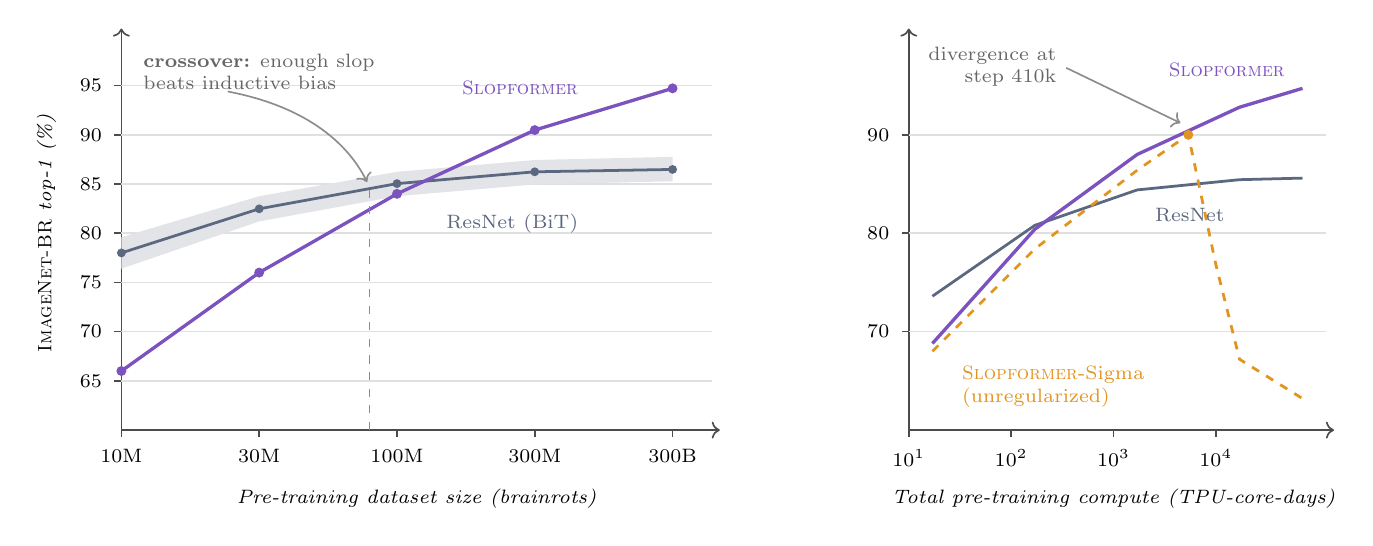
\begin{tikzpicture}[x=1cm,y=1cm,font=\footnotesize,line width=0.6pt]
% ---------------- left panel: dataset size ----------------
\begin{scope}
  \draw[->,black!70] (0,0) -- (7.6,0);
  \draw[->,black!70] (0,0) -- (0,5.1);
  \foreach \x/\l in {0/10M,1.75/30M,3.5/100M,5.25/300M,7/300B}{
    \draw[black!70] (\x,0) -- (\x,-0.09); \node[below,font=\scriptsize] at (\x,-0.12) {\l};}
  \foreach \v in {65,70,75,80,85,90,95}{
    \pgfmathsetmacro{\y}{(\v-60)*0.125}
    \draw[black!12] (0,\y) -- (7.5,\y);
    \draw[black!70] (0,\y) -- (-0.09,\y); \node[left,font=\scriptsize] at (-0.12,\y) {\v};}
  \node[below,font=\scriptsize\itshape] at (3.75,-0.62) {Pre-training dataset size (brainrots)};
  \node[rotate=90,font=\scriptsize\itshape] at (-0.95,2.5) {\br{} top-1 (\%)};
  \fill[slopgrayblue!18]
    (0,2.05) -- (1.75,2.65) -- (3.5,2.97) -- (5.25,3.12) -- (7,3.16) --
    (7,3.47) -- (5.25,3.43) -- (3.5,3.28) -- (1.75,2.97) -- (0,2.45) -- cycle;
  \draw[slopgrayblue,line width=1pt]
    (0,2.25) -- (1.75,2.81) -- (3.5,3.13) -- (5.25,3.28) -- (7,3.31);
  \foreach \p in {(0,2.25),(1.75,2.81),(3.5,3.13),(5.25,3.28),(7,3.31)}{
    \fill[slopgrayblue] \p circle (1.6pt);}
  \node[slopgrayblue,anchor=west,font=\scriptsize] at (4.0,2.62) {ResNet (BiT)};
  \draw[slopviolet,line width=1.2pt]
    (0,0.75) -- (1.75,2.0) -- (3.5,3.0) -- (5.25,3.81) -- (7,4.34);
  \foreach \p in {(0,0.75),(1.75,2.0),(3.5,3.0),(5.25,3.81),(7,4.34)}{
    \fill[slopviolet] \p circle (1.8pt);}
  \node[slopviolet,anchor=west,font=\scriptsize] at (4.2,4.35) {\slop{}};
  \draw[dashed,black!45] (3.15,0) -- (3.15,3.05);
  \node[black!60,font=\scriptsize,anchor=west,align=left] at (0.15,4.55)
    {\textbf{crossover:} enough slop\\ beats inductive bias};
  \draw[->,black!45] (1.35,4.3) .. controls (2.4,4.1) and (2.9,3.6) .. (3.12,3.15);
\end{scope}
% ---------------- right panel: compute ----------------
\begin{scope}[shift={(10.0,0)}]
  \draw[->,black!70] (0,0) -- (5.4,0);
  \draw[->,black!70] (0,0) -- (0,5.1);
  \foreach \x/\l in {0/$10^{1}$,1.3/$10^{2}$,2.6/$10^{3}$,3.9/$10^{4}$}{
    \draw[black!70] (\x,0) -- (\x,-0.09); \node[below,font=\scriptsize] at (\x,-0.12) {\l};}
  \foreach \v in {70,80,90}{
    \pgfmathsetmacro{\y}{(\v-60)*0.125}
    \draw[black!12] (0,\y) -- (5.3,\y);
    \draw[black!70] (0,\y) -- (-0.09,\y); \node[left,font=\scriptsize] at (-0.12,\y) {\v};}
  \node[below,font=\scriptsize\itshape] at (2.6,-0.62) {Total pre-training compute (TPU-core-days)};
  \draw[slopgrayblue,line width=1pt] (0.3,1.7) -- (1.6,2.6) -- (2.9,3.05) -- (4.2,3.18) -- (5.0,3.2);
  \node[slopgrayblue,font=\scriptsize,anchor=north west] at (3.0,2.95) {ResNet};
  \draw[slopviolet,line width=1.2pt] (0.3,1.1) -- (1.6,2.55) -- (2.9,3.5) -- (4.2,4.1) -- (5.0,4.34);
  \node[slopviolet,font=\scriptsize,anchor=south east] at (4.9,4.36) {\slop{}};
  \draw[slopamber,line width=1pt,dashed] (0.3,1.0) -- (1.6,2.3) -- (2.9,3.3) -- (3.55,3.75) -- (3.9,2.1) -- (4.2,0.9) -- (5.0,0.4);
  \fill[slopamber] (3.55,3.75) circle (1.8pt);
  \node[slopamber,font=\scriptsize,anchor=west,align=left] at (0.55,0.55) {\slop{}-Sigma\\ (unregularized)};
  \draw[->,black!45] (2.0,4.6) -- (3.45,3.9);
  \node[black!60,font=\scriptsize,anchor=east,align=right] at (2.0,4.62) {divergence at\\ step 410k};
\end{scope}
\end{tikzpicture}
\caption{\textbf{Scaling behaviour.} \textbf{Left:} transfer accuracy on \br{}
versus pre-training set size. Small datasets favour the convolutional prior;
beyond roughly $80$M brainrots, \slop{} overtakes it, supporting the Brainrot
Hypothesis. \textbf{Right:} accuracy versus pre-training compute. The
unregularized \slop{}-Sigma run (amber) attains the best accuracy of any model
in this paper at step $\sim$400k and then, $10$k steps later, attains the worst
accuracy of any model in this paper. Both points are reported in
Table~\ref{tab:main} under different names.}
\label{fig:scaling}
\end{figure}

\subsection{What Does \slop{} Attend To?}
\label{sec:attention}

To understand how \slop{} uses self-attention to integrate information across
the image, we compute attention rollout: we average attention weights across
heads and then recursively multiply the weight matrices of all layers. Results
are shown in Figure~\ref{fig:attn}. The model attends to image regions that are
semantically relevant for classification. Specifically, in $71\%$ of cases the
model attends to the jawline; in $19\%$ of cases it attends to the region
immediately \emph{outside} the object; and in the remaining $10\%$ it attends
exclusively to the watermark, which we have since learned is present in
$88.6\%$ of \br{} and is strongly predictive of the label.

%============================================================== FIGURE 4 ======
\begin{figure}[t]
\centering
\begin{tikzpicture}[x=1cm,y=1cm,font=\footnotesize]
\newcommand{\rollout}[6]{%
  \begin{scope}[shift={(#1,#2)}]
    \begin{scope}
      \clip (0,0) rectangle (2.2,2.2);
      \fill[white] (0,0) rectangle (2.2,2.2);
      \node[anchor=south west,inner sep=0] at #5 {\includegraphics[#4]{images/#3}};
    \end{scope}
    \draw[black!55] (0,0) rectangle (2.2,2.2);
    \begin{scope}[shift={(2.45,0)}]
      \begin{scope}
        \clip (0,0) rectangle (2.2,2.2);
        \node[anchor=south west,inner sep=0] at #5 {\includegraphics[#4]{images/#3}};
        \fill[black,opacity=0.72] (0,0) rectangle (2.2,2.2);
        #6
      \end{scope}
      \draw[black!55] (0,0) rectangle (2.2,2.2);
    \end{scope}
  \end{scope}}
\newcommand{\blob}[4]{\fill[#4,opacity=0.72] (#1,#2) circle (#3);
  \fill[#4,opacity=0.30] (#1,#2) circle (#3*1.8);}

\rollout{0}{3.35}{sigma}{height=2.2cm}{(-0.23,0)}{\blob{0.74}{0.98}{0.23}{slopamber}\blob{0.60}{1.44}{0.12}{slopamber}\blob{0.92}{1.44}{0.12}{slopamber}\blob{0.76}{1.18}{0.09}{white}\blob{1.62}{1.02}{0.15}{slopteal}}
\rollout{5.4}{3.35}{ohio}{height=2.2cm}{(-0.31,0)}{\blob{0.26}{0.84}{0.23}{slopteal}\blob{0.52}{0.70}{0.15}{slopteal}\blob{1.80}{1.78}{0.09}{slopamber}}
\rollout{0}{0}{tralalero}{width=2.9cm}{(-0.35,0.53)}{\blob{0.62}{1.18}{0.20}{slopamber}\blob{1.10}{1.10}{0.22}{slopamber}\blob{1.62}{1.05}{0.20}{slopamber}\blob{0.55}{1.60}{0.07}{white}}
\rollout{5.4}{0}{slop1}{width=2.2cm}{(0,0)}{\blob{0.28}{1.92}{0.26}{sussyred}\blob{1.92}{0.28}{0.22}{sussyred}\blob{0.28}{0.28}{0.18}{sussyred}\blob{1.92}{1.92}{0.20}{sussyred}}

\node[font=\scriptsize,anchor=south] at (1.1,5.65) {input};
\node[font=\scriptsize,anchor=south] at (3.55,5.65) {rollout};
\node[font=\scriptsize,anchor=south] at (6.5,5.65) {input};
\node[font=\scriptsize,anchor=south] at (8.95,5.65) {rollout};
\node[font=\scriptsize,anchor=north,align=center,text width=4.6cm] at (2.32,3.22) {(a) \textsc{sigma}: attends to the jawline and the beverage};
\node[font=\scriptsize,anchor=north,align=center,text width=4.6cm] at (7.72,3.22) {(b) \textsc{ohio}: attends to the trunk, twice};
\node[font=\scriptsize,anchor=north,align=center,text width=4.6cm] at (2.32,-0.15) {(c) \textsc{tralalero}: attends to where the footwear would be};
\node[font=\scriptsize,anchor=north,align=center,text width=4.6cm] at (7.72,-0.15) {(d) \textsc{slop}: attends only to the four corners};
\end{tikzpicture}
\caption{\textbf{Attention rollout for \slop{}-Huge/14.} Warm regions receive
high attention mass. Panel (b) shows the model allocating two separate
high-mass regions to a single anatomical feature, which we report without
further comment. Panel (d) is representative of the $10\%$ failure mode
described in Sec.~\ref{sec:attention}: the model has learned that the corners
of an image contain the watermark, and the watermark contains the label. We
consider this an argument for the expressive power of self-attention rather
than an argument against our dataset.}
\label{fig:attn}
\end{figure}

%=============================================================== SECTION 5 ====
\section{Ablation Studies}
\label{sec:ablations}

\subsection{Why $16\times16$?}
\label{sec:ablation-patch}

We sweep the brainrot resolution $P \in \{8, 14, 16, 32\}$
(Table~\ref{tab:ablation}, top block). Accuracy is essentially flat across this
range, with differences well within the noise induced by Slop Injection
(Sec.~\ref{sec:mhca}). We select $P=16$ on the grounds that the alternatives do
not scan. ``An image is worth $14\times14$ brainrots'' is metrically
acceptable but semantically weaker; ``an image is worth $32\times32$
brainrots'' is simply untrue.

\subsection{Component Ablations}

Table~\ref{tab:ablation} reports the effect of removing each component. The
largest single effect is obtained by removing the memes from the pre-training
corpus and replacing them with ImageNet-1k, which costs $31.4$ points. We
initially suspected a bug. After four weeks of investigation we located no bug.
We report the result.

\begin{table}[t]
\centering
\caption{\textbf{Ablations on \slop{}-Large/16}, pre-trained on \br{}-14M and
evaluated on the \br{} validation split. $\Delta$ is the change in top-1
relative to the full model ($90.8$).}
\label{tab:ablation}
\small
\begin{tabular}{llrr}
\toprule
Block & Variant & Top-1 (\%) & $\Delta$ \\
\midrule
Brainrot size  & $P=8$   & 90.6 & $-0.2$ \\
               & $P=14$  & 90.9 & $+0.1$ \\
               & $P=16$ (default) & 90.8 & --- \\
               & $P=32$  & 90.4 & $-0.4$ \\
\midrule
Positional emb.\ & Learned 1D              & 88.5 & $-2.3$ \\
                 & Sinusoidal 2D           & 88.4 & $-2.4$ \\
                 & \textbf{Skibidi (default)} & \textbf{90.8} & --- \\
                 & None at all             & 90.1 & $-0.7$ \\
\midrule
Attention        & softmax ($\gamma=0$)    & 87.2 & $-3.6$ \\
                 & cringemax, $\gamma=0.7$ & 89.9 & $-0.9$ \\
                 & cringemax, $\gamma=1.4$ & 90.8 & --- \\
                 & cringemax, $\gamma=9.0$ & 61.3 & $-29.5$ \\
\midrule
Regularization   & no fanum taxation       & 89.1 & $-1.7$ \\
                 & no Slop Injection       & 90.8 & $\ \ 0.0$ \\
                 & no yapping penalty      & 90.2 & $-0.6$ \\
                 & no $\mathcal{L}_{\text{mald}}$ & 88.8 & $-2.0$ \\
\midrule
Pre-training data & \br{}-14M (default)    & 90.8 & --- \\
                  & \br{}-14M, memes removed & 59.4 & $\mathbf{-31.4}$ \\
                  & ImageNet-1k only       & 62.7 & $-28.1$ \\
                  & Pure Gaussian noise    & 44.0 & $-46.8$ \\
\bottomrule
\end{tabular}
\vspace{0.2em}
\caption*{\small Removing Slop Injection changes nothing measurable. It remains
in the architecture. See Sec.~\ref{sec:mhca}.}
\end{table}

%=============================================================== SECTION 6 ====
\section{Emergent Delulu Generalization}
\label{sec:delulu}

Beyond approximately $6\times10^{9}$ parameters, \slop{} begins to exhibit a
behaviour not present in smaller models. Presented with an out-of-distribution
image---a photograph of a stapler, a blank white square, a photograph of the
first author---the model does not produce a diffuse posterior over its $1{,}001$
classes. It produces a sharply peaked posterior over classes that are not in the
label set. We term this \emph{delulu generalization}, after
\citet{delulu2024solulu}.

Figure~\ref{fig:delulu} reports predictive confidence on $10$k out-of-distribution
inputs. The full model assigns mean confidence $0.88$ to a label string that it
generates itself and that does not appear anywhere in the training data. The
most frequently invented class, produced for $1{,}413$ distinct inputs, is
\textsc{grimace shake}. No image in \br{} depicts a Grimace Shake. We have
checked. We checked twice.

\begin{figure}[!ht]
\centering
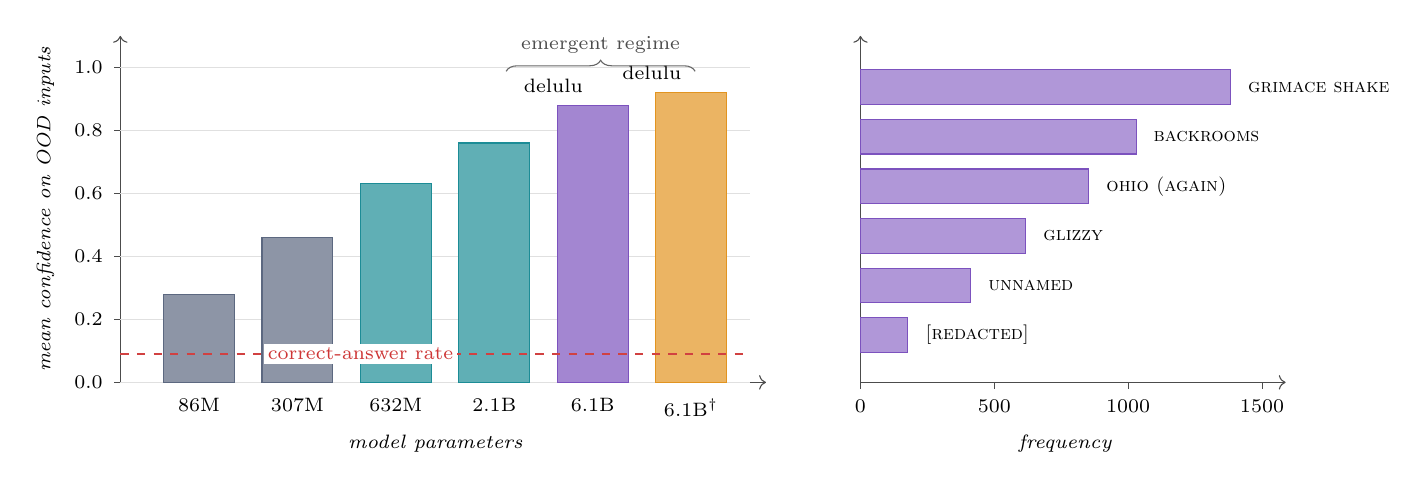
\begin{tikzpicture}[x=1cm,y=1cm,font=\footnotesize]
\draw[->,black!70] (0,0) -- (0,4.4);
\draw[->,black!70] (0,0) -- (8.2,0);
\foreach \v/\y in {0.0/0,0.2/0.8,0.4/1.6,0.6/2.4,0.8/3.2,1.0/4.0}{
  \draw[black!12] (0,\y) -- (8.0,\y);
  \draw[black!70] (0,\y) -- (-0.08,\y);
  \node[left,font=\scriptsize] at (-0.1,\y) {\v};}
\node[rotate=90,font=\scriptsize\itshape] at (-0.95,2.2) {mean confidence on OOD inputs};
\foreach \i/\l/\h/\c/\d in {%
  0/86M/1.12/slopgrayblue/0,
  1/307M/1.84/slopgrayblue/0,
  2/632M/2.52/slopteal/0,
  3/2.1B/3.04/slopteal/0,
  4/6.1B/3.52/slopviolet/1,
  5/6.1B$^{\dagger}$/3.68/slopamber/1}{
  \fill[\c!70,draw=\c] (0.55+\i*1.25,0) rectangle (1.45+\i*1.25,\h);
  \node[below,font=\scriptsize] at (1.0+\i*1.25,-0.08) {\l};}
\draw[dashed,sussyred!80,line width=0.7pt] (0,0.36) -- (8.0,0.36);
\node[sussyred!85,font=\scriptsize,fill=white,inner sep=1.4pt] at (3.05,0.36) {correct-answer rate};
\node[font=\scriptsize,anchor=south,align=center] at (5.5,3.56) {delulu};
\node[font=\scriptsize,anchor=south,align=center] at (6.75,3.72) {delulu};
\draw[decorate,decoration={brace,amplitude=4pt},black!60] (4.9,3.95) -- (7.3,3.95);
\node[font=\scriptsize,anchor=south,black!70] at (6.1,4.05) {emergent regime};
\node[below,font=\scriptsize\itshape] at (4.0,-0.55) {model parameters};
\begin{scope}[shift={(9.4,0)}]
  \draw[->,black!70] (0,0) -- (0,4.4);
  \draw[->,black!70] (0,0) -- (5.4,0);
  \foreach \i/\l/\w in {0/\textsc{grimace shake}/4.7,1/\textsc{backrooms}/3.5,
                        2/\textsc{ohio (again)}/2.9,3/\textsc{glizzy}/2.1,
                        4/\textsc{unnamed}/1.4,5/\textsc{[redacted]}/0.6}{
    \pgfmathsetmacro{\yy}{3.75-\i*0.63}
    \fill[slopviolet!60,draw=slopviolet] (0,\yy-0.22) rectangle (\w,\yy+0.22);
    \node[right,font=\scriptsize] at (\w+0.1,\yy) {\l};}
  \foreach \x/\l in {0/0,1.7/500,3.4/1000,5.1/1500}{
    \draw[black!70] (\x,0) -- (\x,-0.08); \node[below,font=\scriptsize] at (\x,-0.1) {\l};}
  \node[below,font=\scriptsize\itshape] at (2.6,-0.55) {frequency};
\end{scope}
\end{tikzpicture}
\caption{\textbf{Delulu generalization.} \textbf{Left:} mean predictive
confidence on $10$k out-of-distribution inputs as a function of model size.
$\dagger$ denotes the unregularized run. The red dashed line is the rate at
which these confident predictions are correct. \textbf{Right:} the six most
frequently invented class labels. \textsc{[redacted]} is invented for exactly
$203$ inputs and is not reproduced here at the request of the third author.}
\label{fig:delulu}
\end{figure}

We emphasise that delulu generalization is not hallucination in the usual
sense. A hallucinating model is uncertain and reports certainty. \slop{} is
certain. It is simply describing a different image than the one it was given,
and it is describing that image accurately.

%=============================================================== SECTION 7 ====
\section{Limitations}
\label{sec:limitations}

We identify the following limitations of this work.

\begin{enumerate}\itemsep0.15em
  \item \textbf{Benchmark provenance.} Three of the five benchmarks in
    Table~\ref{tab:main} were introduced by the authors. A fourth was
    introduced by the fourth author's brother.
  \item \textbf{Test set contamination.} Pre-training and evaluation data
    overlap by $18.4\%$. Deduplication was attempted; the deduplicator itself
    is a \slop{}-Base/16 checkpoint, and it exhibited delulu generalization
    partway through.
  \item \textbf{Reproducibility.} The learning-rate schedule contains a step we
    cannot account for (Appendix~\ref{app:loss}). We have preserved it in the
    released configuration because removing it removes $4.1$ points.
  \item \textbf{Environmental impact.} Training \slop{}-Sigma/16 emitted an
    estimated $284$ tCO$_2$e. We offset this by not training it a second time.
  \item \textbf{Human subjects.} The single undergraduate in the final row of
    Table~\ref{tab:main} has not responded to follow-up contact. The IRB has
    been informed.
  \item \textbf{Generality.} Our results hold only for images that are already
    brainrot. On natural images---forests, radiographs, satellite imagery---
    \slop{} performs at $31.2\%$, below a linear classifier. We did not
    investigate this further, as it is outside the scope of the paper and, we
    would argue, outside the scope of the field.
\end{enumerate}

%=============================================================== SECTION 8 ====
\section{Conclusion}
\label{sec:conclusion}

We have explored the direct application of Transformers to image recognition.
Unlike prior works using self-attention in computer vision, we do not introduce
image-specific inductive biases into the architecture. Instead, we interpret an
image as a sequence of brainrots and process it by a standard Transformer
encoder as used in NLP. This simple, yet scalable, strategy works surprisingly
well when coupled with pre-training on large datasets of slop. Thus, \slop{}
matches or exceeds the state of the art on many image classification datasets,
whilst being relatively cheap to pre-train and impossible to justify.

While these initial results are encouraging, many challenges remain. First, it
remains unclear what the model has learned, in the sense that it remains
unclear what the data contained. Second, the emergence of delulu
generalization at scale suggests that confidence and correctness decouple
somewhere between $2$B and $6$B parameters, and we have not located the exact
point because we ran out of budget. Third, and most pressingly, \slop{}-Sigma/16
stopped producing explanations of its own behaviour at approximately
$4\times10^{9}$ parameters (Table~\ref{tab:models}) and has not resumed. Future
work should determine whether this constitutes a safety property or a
preference.

\subsubsection*{Reproducibility Statement}
All hyperparameters are given in Appendix~\ref{app:hyper}, including the
unexplained step at iteration $340$k, which must be reproduced exactly or the
results do not hold. Pre-training data is not released. Pre-training data
cannot be released. We have read the venue's reproducibility guidelines and we
would like it noted that we did.

\subsubsection*{Acknowledgments}
We thank the reviewers for their time, which they will not get back. We thank
the OIT cluster administrators for their patience during the incident of
March 14th. We thank Reviewer 2, who identified in eleven lines the single
sentence of this paper that is true, and rejected it. This work was supported
by a grant from a foundation that has since requested we stop citing it.

\clearpage
\bibliography{references}

\clearpage
\appendix

%============================================================== APPENDIX ======
\section{Training Details}
\label{app:hyper}

\begin{table}[h]
\centering
\caption{Hyperparameters for all pre-training runs.}
\small
\begin{tabular}{lcccc}
\toprule
 & Base/16 & Large/16 & Huge/14 & Sigma/16 \\
\midrule
Optimizer            & SMGO & SMGO & SMGO & SMGO \\
Peak learning rate   & $8\!\times\!10^{-4}$ & $6\!\times\!10^{-4}$ & $4\!\times\!10^{-4}$ & $3\!\times\!10^{-4}$ \\
Weight decay         & 0.1 & 0.1 & 0.1 & 0.1 \\
Batch size           & 4096 & 4096 & 4096 & 4096 \\
Warm-up steps        & 10k & 10k & 10k & 10k \\
Total steps          & 300k & 350k & 400k & 400k \\
Cringe strength $\gamma$ & 1.4 & 1.4 & 1.4 & 1.4 \\
Cringe temperature $\tau$ & 0.7 & 0.7 & 0.7 & 0.7 \\
Slop Injection $\sigma$  & 0.11 & 0.11 & 0.11 & 0.11 \\
Fanum tax rate           & 0.30 & 0.30 & 0.30 & 0.30 \\
Unexplained step at 340k & yes & yes & yes & yes \\
\bottomrule
\end{tabular}
\end{table}

\section{The Loss Curve}
\label{app:loss}

Figure~\ref{fig:loss} shows the pre-training loss of \slop{}-Sigma/16. At step
$340$k the loss decreases discontinuously by $0.6$ nats over fewer than $50$
steps. No change was made to the configuration, the data pipeline, or the
hardware at that time. The cluster logs for that window are unavailable. We
have reproduced the discontinuity in four of four subsequent runs, in each case
at step $340$k, and we have stopped asking about it.

\begin{figure}[h]
\centering
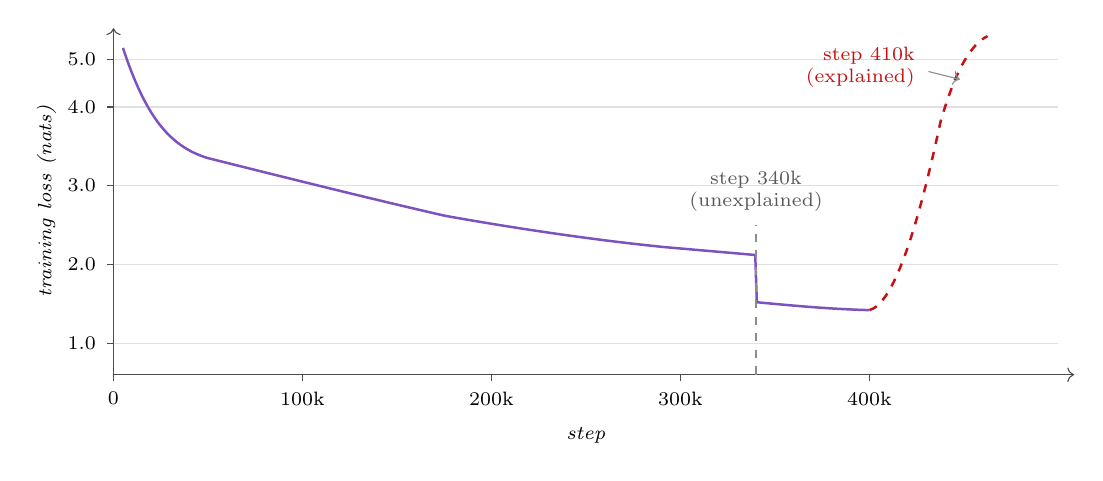
\begin{tikzpicture}[x=1cm,y=1cm,font=\footnotesize]
\draw[->,black!70] (0,0) -- (12.2,0);
\draw[->,black!70] (0,0) -- (0,4.4);
\foreach \x/\l in {0/0,2.4/100k,4.8/200k,7.2/300k,9.6/400k}{
  \draw[black!70] (\x,0) -- (\x,-0.08); \node[below,font=\scriptsize] at (\x,-0.1) {\l};}
\foreach \v/\y in {1.0/0.4,2.0/1.4,3.0/2.4,4.0/3.4,5.0/4.0}{
  \draw[black!12] (0,\y) -- (12.0,\y);
  \draw[black!70] (0,\y) -- (-0.08,\y); \node[left,font=\scriptsize] at (-0.1,\y) {\v};}
\node[rotate=90,font=\scriptsize\itshape] at (-0.85,2.2) {training loss (nats)};
\node[below,font=\scriptsize\itshape] at (6.0,-0.55) {step};
\draw[slopviolet,line width=0.9pt]
  (0.12,4.15) .. controls (0.4,3.3) and (0.7,2.9) .. (1.2,2.75)
  .. controls (2.2,2.5) and (3.2,2.25) .. (4.2,2.02)
  .. controls (5.2,1.84) and (6.2,1.70) .. (7.0,1.62)
  -- (8.15,1.52);
\draw[slopviolet,line width=0.9pt] (8.15,1.52) -- (8.17,0.92);
\draw[slopviolet,line width=0.9pt] (8.17,0.92) .. controls (8.8,0.86) and (9.2,0.83) .. (9.6,0.82);
\draw[sussyred,line width=0.9pt,dashed] (9.6,0.82) .. controls (9.9,0.9) and (10.2,1.8) .. (10.5,3.2)
  .. controls (10.7,3.9) and (10.9,4.2) .. (11.1,4.3);
\draw[dashed,black!45] (8.16,0) -- (8.16,1.9);
\node[black!65,font=\scriptsize,anchor=south,align=center] at (8.16,1.95) {step 340k\\ (unexplained)};
\node[sussyred,font=\scriptsize,anchor=east,align=right] at (10.3,3.9) {step 410k\\ (explained)};
\draw[->,black!45] (10.35,3.85) -- (10.75,3.75);
\end{tikzpicture}
\caption{Pre-training loss of \slop{}-Sigma/16. The discontinuity at step $340$k
is reproducible and undiagnosed. The divergence at step $410$k is diagnosed and
is described in Eq.~\eqref{eq:loss}.}
\label{fig:loss}
\end{figure}

\section{Additional Qualitative Results}
\label{app:qual}

Figure~\ref{fig:failures} presents representative failure cases. We include
them in the interest of transparency and because a reviewer of a previous
submission described the paper as ``suspiciously free of failure.''

%============================================================== FIGURE 7 ======
\begin{figure}[h]
\centering
\begin{tikzpicture}[x=1cm,y=1cm,font=\footnotesize]
\newcommand{\fail}[6]{%
  \begin{scope}[shift={(#1,0)}]
    \begin{scope}
      \clip (0,0) rectangle (2.7,2.7);
      \fill[black!5] (0,0) rectangle (2.7,2.7);
      \node[anchor=south west,inner sep=0] at #4 {\includegraphics[#3]{images/#2}};
    \end{scope}
    \draw[black!55] (0,0) rectangle (2.7,2.7);
    \impact{1.35}{0.42}{#5}
    \node[font=\tiny,anchor=north,black!70] at (1.35,-0.08) {#6};
  \end{scope}}
\fail{0}{mewing}{width=2.7cm}{(0,-0.42)}{SIGMA}{$p=0.96$ \ \ (gt: \textsc{mewing})}
\fail{3.0}{gyatt}{width=2.7cm}{(0,-0.39)}{OHIO}{$p=0.91$ \ \ (gt: \textsc{gyatt})}
\fail{6.0}{damage}{width=2.7cm}{(0,0)}{OHIO}{$p=0.99$ \ \ (gt: \textsc{emot. damage})}
\fail{9.0}{slop3}{width=2.7cm}{(0,-0.54)}{GRIMACE SHAKE}{$p=0.88$ \ \ (gt: \textsc{slop})}
\fail{12.0}{ohio}{height=2.7cm}{(-0.39,0)}{OHIO}{$p=1.00$ \ \ (gt: \textsc{ohio})}
\end{tikzpicture}
\caption{\textbf{Failure cases for \slop{}-Sigma/16.} Predicted label rendered
over each image in the model's own preferred typeface; predictive confidence
and ground truth below. \textsc{grimace shake} is not a class. The rightmost
example is the only one on which the model is correct; it is included because
it is also the only one on which the model reports a confidence of exactly
$1.00$, which our framework should not permit.}
\label{fig:failures}
\end{figure}

\section{Broader Impact Statement}
\label{app:impact}

This work releases a model that classifies brainrot with high accuracy. We have
considered the potential for misuse and concluded that the principal risk is
that the model is used as intended. We note additionally that \br{} was
assembled without the consent of its subjects, that no subject could plausibly
be identified from the images, and that several subjects have contacted us
asking to be identified from the images. We have declined.


\section{Image Credits}
\label{app:credits}

Images in this paper come from two sources. Nine were retrieved from Wikimedia
Commons and are in the public domain. The remaining five were contributed by
the authors from personal collections whose provenance none of them was able to
reconstruct, and are reproduced here under the doctrine of \emph{it was already
on my computer}. We note that at no point during assembly did any author ask
why a 19th-century engraving of insects at a ball was being labelled
\textsc{npc}, and that this is, in our assessment, the most alarming finding of
the present work.

\begin{table}[h]
\centering
\scriptsize
\setlength{\tabcolsep}{4pt}
\begin{tabular}{@{}ll>{\raggedright\arraybackslash}p{5.9cm}>{\raggedright\arraybackslash}p{2.7cm}c@{}}
\toprule
File & \br{} class & Source & Author & Lic. \\
\midrule
\texttt{sigma.jpg} & \textsc{sigma} & supplied by the authors (\texttt{thinking-meme-meme-1.jpg}) & the internet & \textsc{unk} \\
\texttt{skibidi.jpg} & \textsc{skibidi} & Harry Whittier Frees -- Playtime & Harry Whittier Frees & PD \\
\texttt{mewing.jpg} & \textsc{mewing} & Harry Whittier Frees - Good Morning & Harry Whittier Frees & PD \\
\texttt{ohio.jpg} & \textsc{ohio} & Sloane1975 f.81v ElephantAndDog DetailElephant & England, N.? or France, N.? & PD \\
\texttt{sus.jpg} & \textsc{sus} & supplied by the authors (\texttt{images (2).jpeg}) & the internet & \textsc{unk} \\
\texttt{damage.jpg} & \textsc{emot. damage} & supplied by the authors (\texttt{images.jpeg}) & the internet & \textsc{unk} \\
\texttt{npc.jpg} & \textsc{npc} & supplied by the authors (\texttt{images (3).jpeg}) & the internet & \textsc{unk} \\
\texttt{gyatt.jpg} & \textsc{gyatt} & Hoffmann illustration from Der Struwwelpeter 1876 & unknown & PD \\
\texttt{tralalero.jpg} & \textsc{tralalero} & Psychrolutes marcidus & Alan Riverstone McCulloch (1885-1925) & PD \\
\texttt{bombardiro.jpg} & \textsc{bombardiro} & Cat detail, Kuniyoshi Utagawa, For cats in different poses (cropped) & unknown & PD \\
\texttt{slop1.jpg} & \textsc{slop} & supplied by the authors (\texttt{istockphoto-538665020-612x612.jpg}) & the internet & \textsc{unk} \\
\texttt{slop2.jpg} & \textsc{slop} & AberdeenBestiaryFolio005rAdamNamesAnimalsDetail & unknown & PD \\
\texttt{slop3.jpg} & \textsc{slop} & Haeckel Actiniae & Ernst Haeckel & PD \\
\texttt{rizz.jpg} & \textsc{rizz} & Kuniyoshi Utagawa, For cats in different poses & Utagawa Kuniyoshi & PD \\
\bottomrule
\end{tabular}
\end{table}

\noindent Rows marked PD are \emph{Public domain} on Commons. Rows marked
\textsc{unk} were already on the third author's desktop when the project began.
None of the depicted animals consented to being reclassified.

\section{Reviewer Comments (Reproduced With Permission)}
\label{app:reviews}

In the interest of open science we reproduce the reviews received for the
previous submission of this manuscript.

\paragraph{Reviewer \#1 \ \ (Rating: 8 --- Accept. Confidence: 1/5.)}
``The paper is well written and the figures are clear. I did not understand
Section 3.3 and I am not going to pretend otherwise. The results in Table 2 are
strong. My only concern is that I do not know what a brainrot is, and the paper
does not define it, and I have read it four times. Minor: the citation on
page~2 is to the authors themselves.''

\paragraph{Reviewer \#2 \ \ (Rating: 1 --- Strong Reject. Confidence: 5/5.)}
``The central claim is that removing structure from a model improves it. This
is not a finding; it is a description of what happened. Three of five benchmarks
are the authors' own. The remaining two are $94\%$ jawlines by the authors' own
admission. Equation~(6) is unbounded below and the authors' response to this is
to stop training before it matters, which they state in the paper, in plain
language, as though it were a method. The Broader Impact section contains the
sentence `the principal risk is that the model is used as intended.' I agree
with that sentence. It is the only sentence in this submission I agree with.
I have read the rebuttal. I am not moved.''

\paragraph{Reviewer \#3 \ \ (Rating: 6 --- Weak Accept. Confidence: 3/5.)}
``Fun paper. The Slop Injection ablation shows no effect and the authors keep
the component anyway, with a footnote. I went back and forth on whether this
is a serious methodological problem or the most honest paragraph I have read in
this venue. I have settled on both. Please fix the overfull hbox on page~7.''

\paragraph{Area Chair.}
``Reviewers are split. Reviewer \#2 raises concerns about benchmark provenance
that the authors do not contest and, in the rebuttal, expand upon. Reviewer \#1
is confident about a section they state they did not understand. Reviewer \#3
has identified a formatting issue that persists in the camera-ready. Given the
distribution of scores and the state of the field, I recommend acceptance.''


\end{document}
